%%%%%%%%%%%%%%%%%%%%%%%%%%%%%%%%%%%%%%%%%
% Class Notes Template
% LaTeX Template
% By: Ryan Grove
%%%%%%%%%%%%%%%%%%%%%%%%%%%%%%%%%%%%%%%%%

%----------------------------------------------------------------------------------------
%	PACKAGES AND OTHER DOCUMENT CONFIGURATIONS
%----------------------------------------------------------------------------------------

\documentclass[paper=a4, fontsize=11pt]{scrartcl} % A4 paper and 11pt font size

\usepackage[T1]{fontenc} % Use 8-bit encoding that has 256 glyphs
\usepackage{fourier} % Use the Adobe Utopia font for the document - comment this line to return to the LaTeX default
\usepackage[english]{babel} % English language/hyphenation
\usepackage{amsmath,amsfonts,amsthm} % Math packages

\usepackage{lipsum} % Used for inserting dummy 'Lorem ipsum' text into the template

\usepackage{sectsty} % Allows customizing section commands
\allsectionsfont{\centering \normalfont\scshape} % Make all sections centered, the default font and small caps

\usepackage{fancyhdr} % Custom headers and footers
\pagestyle{fancyplain} % Makes all pages in the document conform to the custom headers and footers
\fancyhead{} % No page header - if you want one, create it in the same way as the footers below
\fancyfoot[L]{} % Empty left footer
\fancyfoot[C]{} % Empty center footer
%\fancyfoot[R]{\thepage} % Page numbering for right footer
\renewcommand{\headrulewidth}{0pt} % Remove header underlines
\renewcommand{\footrulewidth}{0pt} % Remove footer underlines
\setlength{\headheight}{13.6pt} % Customize the height of the header

\numberwithin{equation}{section} % Number equations within sections (i.e. 1.1, 1.2, 2.1, 2.2 instead of 1, 2, 3, 4)
\numberwithin{figure}{section} % Number figures within sections (i.e. 1.1, 1.2, 2.1, 2.2 instead of 1, 2, 3, 4)
\numberwithin{table}{section} % Number tables within sections (i.e. 1.1, 1.2, 2.1, 2.2 instead of 1, 2, 3, 4)

\setlength\parindent{0pt} % Removes all indentation from paragraphs - comment this line for an assignment with lots of text

\usepackage{lastpage}
\usepackage{fancyhdr}
\cfoot{\thepage\ of \pageref{LastPage}}

\def\v{\hbox{$\mathbf v$}}
\def\w{\hbox{$\mathbf w$}}
\def\u{\hbox{$\mathbf u$}}
\def\x{\hbox{$\textbf{x}$}}
\def\z{\hbox{$\mathbf z$}}
\def\a{\hbox{$\mathbf a$}}
\def\b{\hbox{$\mathbf b$}}
\def\L{\hbox{$\mathcal L$}}
\def\C{\hbox{$\mathbb C$}}
\def\B{\hbox{$\mathcal B$}}
\def\R{\hbox{$\mathbb R$}}
\def\X{\hbox{$\underline X$}}
\def\Q{\hbox{$\mathbb Q$}}
\def\R{\hbox{$\mathbb R$}}
\def\N{\hbox{$\mathbb N$}}
\def\C{\hbox{$\mathbb C$}}
\def\0{\hbox{$\mathbf 0$}}
\def\Y{\hbox{$\underline Y$}}
\def\a{\hbox{$\mathbf a$}}
\def\u{\hbox{$\mathbf u$}}
\def\w{\hbox{$\mathbf w$}}
\def\y{\hbox{$\mathbf y$}}
\def\X{\hbox{$\underline X$}}
\def\dd{\hbox{$\partial $}}
\def\B{\hbox{$\mathcal B$}}
\def\F{\hbox{$\mathcal F$}}
\def\L{\hbox{$\mathcal L$}}
\def\M{\hbox{$\mathcal M$}}
\def\D{\hbox{$\mathscr {D}$}}
\def\RR{\hbox{$\mathscr{R}$}}
\def\I{\hbox{$\mathcal I$}}

\usepackage{amssymb}
%\theoremstyle{plain}
\usepackage[margin = .75in]{geometry}
\newtheorem{claim}{Claim}
\newtheorem{theorem}{Theorem}[section]
\newtheorem{lemma}[theorem]{Lemma}
\newtheorem{proposition}[theorem]{Proposition}
\newtheorem{corollary}[theorem]{Corollary}
\newtheorem{problem}[theorem]{Problem}
%\theoremstyle{definition}
\newtheorem{definition}[theorem]{Definition}
%\theoremstyle{remark}
\newtheorem{remark}[theorem]{Remark}
\newtheorem{remarks}[theorem]{Remarks}
\newtheorem{example}[theorem]{Example}
\newcommand{\ds}{\displaystyle}
\newcommand{\ZZ}{\mathbb{Z}}
\newcommand{\QQ}{\mathbb{Q}}
\newcommand{\e}{\varepsilon}
\newcommand{\bbf}{\textbf}
\newcommand{\p}{\parallel}
\usepackage{color}
\newcommand{\field}[1]{\mathbb{#1}}
\usepackage{amsmath}
\usepackage{amsthm}
\usepackage{amssymb}
\usepackage{mathrsfs}
\usepackage{cancel}
\usepackage{upgreek}
\usepackage{graphicx}
\usepackage{multirow}
\usepackage{setspace}
\usepackage{url}
\usepackage{subfigure}
\usepackage{enumerate}
\usepackage{cases}
\usepackage{mathrsfs}
\usepackage{rotating}

%----------------------------------------------------------------------------------------
%	TITLE SECTION
%----------------------------------------------------------------------------------------

\newcommand{\horrule}[1]{\rule{\linewidth}{#1}} % Create horizontal rule command with 1 argument of height

\title{	
\normalfont \normalsize 
\textsc{Ryan Grove, Clemson University, MATH1080 - 9} \\ [25pt] % Your name, university, class
\horrule{0.5pt} \\[0.4cm] % Thin top horizontal rule
\huge Section 11.8: Power Series\\ % The assignment title
\horrule{2pt} \\[0.5cm] % Thick bottom horizontal rule
}

\author{Date:} % The due date

\date{\normalsize March 23, 2016} % A custom date

\begin{document}

\maketitle % Print the title

\begin{flushleft}
\begin{tabular}{l l}
Name: \rule{3.2in}{.01cm}  & {}%Table number: \rule{1in}{.01cm}\\
\end{tabular}
\end{flushleft}

%----------------------------------------------------------------------------------------
%	Lecture
%----------------------------------------------------------------------------------------

\section*{\textbf{Lecture:}}
A \underline{\hspace{1in}} \underline{\hspace{1in}} is a series of the form

\[\ds\sum_{n=0}^\infty c_n x^n = c_0 + c_1 x + c_2 x^2 + c_3 x^3 + \cdots \hspace{1in} (1)\]

where $x$ is a variable and the $c_n$'s are constants called the \underline{\hspace{1.25in}} of the series. For each fixed $x$, the series $(1)$ is a series of constants that we can test for convergence of divergence. A power series may converge for some values of $x$ and diverge for other values of $x$. The sum of the series is a function
\[f(x) = c_0 + c_1 x + c_2 x^2 + \cdots + c_nx_n + \cdots\]

whose domain is the set of all $x$ for which the series converges. Notice that $f$ resembles a polynomial. The only difference is that $f$ has infinitely many terms.\\
\indent

For instance, if we take $c_n=1$ for all $n$, the power series becomes the geometric series, $\ds\sum_{n=0}^\infty x^n$, which converges when $-1 < x < 1$ and diverges when $|x|\geq 1$.\\
\indent

More generally, a series of the form

\[\ds\sum_{n=0}^\infty c_n (x-a)^n = c_0 + c_1 (x-a) + c_2 (x-a)^2 + \cdots \hspace{1in} (2)\]

is called a \textbf{power series in } \underline{\hspace{1in}} or a \textbf{power series centered at} \underline{\hspace{0.3in}}. Notice that in writing out the term corresponding to $n=0$ in series $(1)$ and $(2)$ above we have adopted the convention that $(x-a)^0=1$ even when $x=a$. Notice also that when $x=a$ all of the terms are 0 for $n\geq 1$ and so the power series $(2)$ \underline{\textbf{ALWAYS}} converges when $\mathbf{x=a}$.\\
\indent

\underline{Example 1}: For what values of $x$ is the series $\ds\sum_{n=0}^\infty n!x^n$ convergent?\\
\indent

\vspace{3in}

\underline{Example 2}: For what values of $x$ does the series $\ds\sum_{n=1}^\infty \ds\frac{(x-3)^n}{n}$ converge?\\
\indent

\vspace{4.75in}

\underline{Example 3}: Find the domain of the Bessel function of order 0 defined by $J_0(x) = \ds\sum_{n=0}^\infty \ds\frac{(-1)^n x^{2n}}{2^{2n}(n!)^2}$.\\
\indent

\vspace{3in}
  
 \fbox{
  \parbox{\textwidth}{
  \vspace{5pt} \textbf{Theorem}: For a given power series $\ds\sum_{n=0}^\infty c_n (x-a)^n$ there are only three possibilities:
  \begin{enumerate}
  \item[(i)] The series converges only when $x=a$.
  \item[(ii)] The series converges for all $x$.
  \item[(iii)] There is a positive number $R$ such that the series converges if $|x-a|<R$ and diverges if $|x-a|>R$.
  \end{enumerate}
  }}
  \indent\\
  \indent
  
  \underline{Definitions}:
  \begin{itemize}
  \item The number $R$ is called the \underline{\hspace{1in}} \underline{\hspace{0.25in}} \underline{\hspace{1.25in}} (ROC) of the power series.\\
  \item The \underline{\hspace{1in}} \underline{\hspace{0.25in}} \underline{\hspace{1.25in}} (IOC) of a power series is the interval that consists of all values of $x$ for which the series converges. 
  \end{itemize}

\vspace{-5pt}
  \[\begin{array}{rll}
  \text{Case } (i):\text{ } &\text{ROC is $R=0$ \quad } &\text{ and } \quad \text{IOC is $\{a\}$}\\
  \text{Case } (ii):\text{ } &\text{ROC is $R=\infty$ }\quad &\text{ and } \quad \text{IOC is $(-\infty,\infty)$}\\
  \text{Case } (iii):\text{ } &\text{ROC is $R$ \text{ }} \quad &\text{ and } \quad \text{IOC is one of the following four:}\\  
    \end{array}\]
    \[(a-R,a+R) \quad \quad (a-R, a+R] \quad \quad [a-R, a+R) \quad \quad [a-R,a+R]\]
  \[\text{*For Case (iii) we must test the \textit{endpoints} $x=a\pm R$.}\]
  \[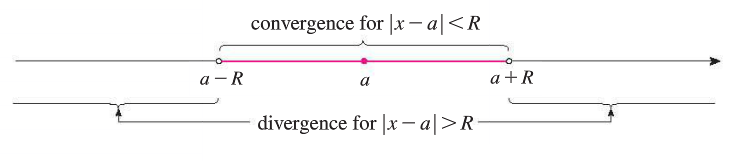
\includegraphics[scale=0.5]{11-8pic1.png}\]
  
  We summarize there the radius and interval of convergence for each of the examples already considered in this section.\\
  
  \[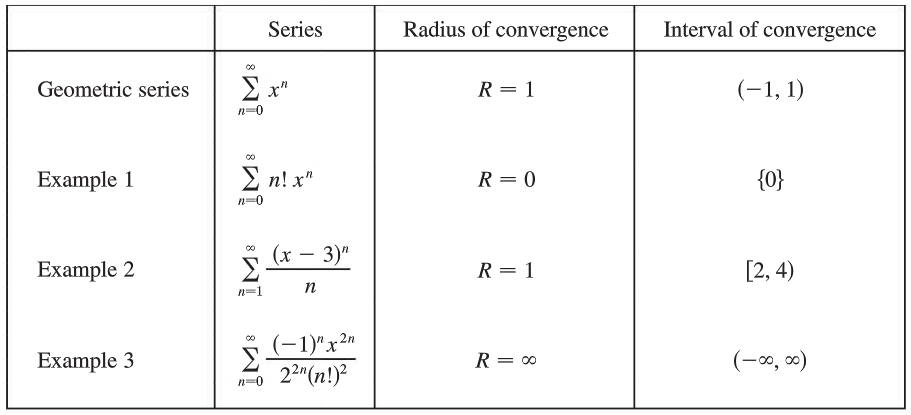
\includegraphics[scale=0.5]{11-8pic2.png}\]
  
  In general, the Ratio Test (or sometimes the Root Test) should be used to determine the radius of convergence $R$. The Ratio and Root Tests always fail when $x$ is an endpoint of the interval of convergence, so the endpoints must be checked with some other test.\\
  \indent
  \newpage
  \underline{Example 4}: Find the radius of convergence and interval of convergence of the series $\ds\sum_{n=0}^\infty \ds\frac{(-3)^n x^n}{\sqrt{n+1}}$.\\
  \indent
  
  \vspace{4in}

  
  \underline{Example 5}: Find the radius of convergence and interval of convergence of the series $\ds\sum_{n=0}^\infty \ds\frac{n(x+2)^n}{3^{n+1}}$.\\
  \indent

%----------------------------------------------------------------------------------------

\end{document}